% Created 2021-10-05 Tue 12:40
% Intended LaTeX compiler: pdflatex
\documentclass[presentation,aspectratio=169, usenames, dvipsnames]{beamer}
\usepackage[utf8]{inputenc}
\usepackage[T1]{fontenc}
\usepackage{graphicx}
\usepackage{grffile}
\usepackage{longtable}
\usepackage{wrapfig}
\usepackage{rotating}
\usepackage[normalem]{ulem}
\usepackage{amsmath}
\usepackage{textcomp}
\usepackage{amssymb}
\usepackage{capt-of}
\usepackage{hyperref}
\usepackage{khpreamble}
\usepackage{amssymb}
\usepgfplotslibrary{groupplots}
\newcommand*{\shift}{\operatorname{q}}
\definecolor{ppc}{rgb}{0.1,0.1,0.6}
\definecolor{iic}{rgb}{0.6,0.1,0.1}
\definecolor{ddc}{rgb}{0.1,0.6,0.1}
\usetheme{default}
\author{Kjartan Halvorsen}
\date{\today}
\title{PID control}
\hypersetup{
 pdfauthor={Kjartan Halvorsen},
 pdftitle={PID control},
 pdfkeywords={},
 pdfsubject={},
 pdfcreator={Emacs 26.3 (Org mode 9.4.6)}, 
 pdflang={English}}
\begin{document}

\maketitle

\section{Integral control example}
\label{sec:org03412a9}

\begin{frame}[label={sec:org11a0c6e}]{Lead-lag compensator for position control of the DC motor}
\begin{center}
 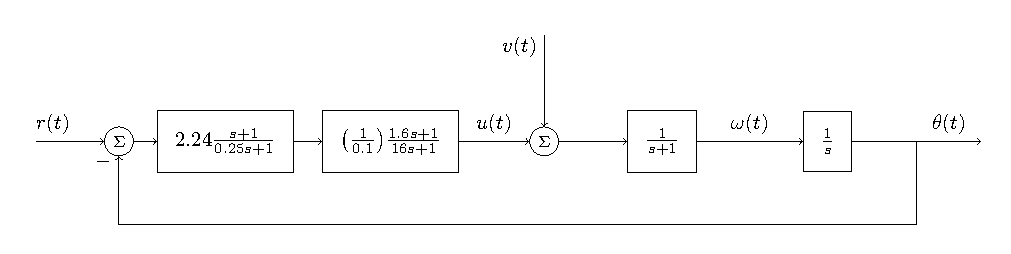
\includegraphics[width=.6\linewidth]{../../figures/block-DC-leadlag-compensator-numerical}
\end{center}

\begin{columns}
\begin{column}{0.5\columnwidth}
\begin{center}
  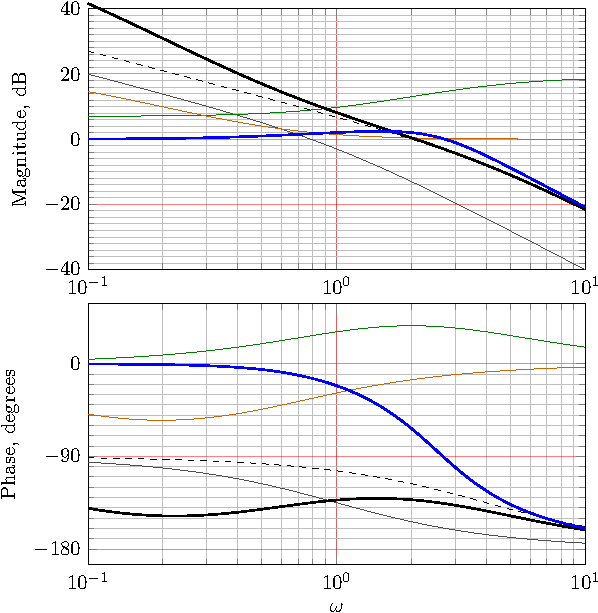
\includegraphics[width=.8\linewidth]{../../figures/bode-loop-gain-leadlag-normalized-DC-crop}
\end{center}
\end{column}


\begin{column}{0.5\columnwidth}
\begin{center}
  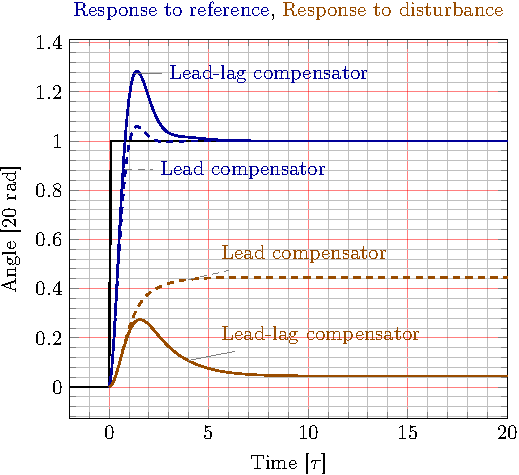
\includegraphics[width=.8\linewidth]{../../figures/response-leadlag-normalized-DC-crop}
\end{center}
\end{column}
\end{columns}
\end{frame}




\section{The need for integral control}
\label{sec:org5b6b53d}

\begin{frame}[label={sec:orgd93ed95}]{Feedback control}
   \begin{center}
   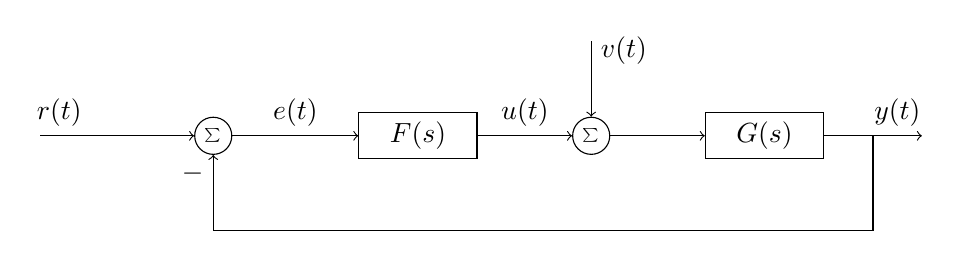
\begin{tikzpicture}[node distance=22mm, block/.style={rectangle, draw, minimum width=15mm}, sumnode/.style={circle, draw, inner sep=2pt}]
  { 
  \node[coordinate] (input) {};
  \node[sumnode, right of=input] (sum) {\tiny $\sum$};
  \node[block, right of=sum, node distance=2.6cm] (reg) {$F(s)$};
  \node[sumnode, right of=reg] (sumd) {\tiny $\sum$};
  \node[block, right of=sumd, node distance=2.2cm] (plant) {$G(s)$};
  \node[coordinate, right of=plant, node distance=2cm] (output) {};
  \node[coordinate, below of=plant, node distance=12mm] (feedback) {};
  \node[coordinate, above of=sumd, node distance=12mm] (dist) {};
 
  \draw[->] (plant) -- node[coordinate, inner sep=0pt] (meas) {} node[near end, above] {$y(t)$} (output);
  \draw[->] (meas) |- (feedback) -| node[very near end, left] {$-$} (sum);
  \draw[->] (input) -- node[very near start, above] {$r(t)$} (sum);
  \draw[->] (sum) -- node[above] {$e(t)$} (reg);
  \draw[->] (reg) -- node[above] {$u(t)$}(sumd);
  \draw[->] (dist) -- node[right, very near start] {$v(t)$}(sumd);
  \draw[->] (sumd) -- node[above] {} (plant);
}
\end{tikzpicture}
\end{center}

\pause

\alert{Activity} What is the transfer function from the load disturbance \(v(t)\) to the control error \(e(t)\)?
\end{frame}


\begin{frame}[label={sec:org61318c1}]{Feedback control - eliminating a constant disturbance}
\small

\[\frac{E(s)}{V(s)} = \frac{-G(s)}{1 + G(s)F(s)} \]

\begin{block}{The final value theorem}
If steady-state exists
\[\lim_{t\to\infty} e(t) = \lim_{s\to 0} sE(s)\]

\pause
\end{block}

\begin{block}{Applied to a constant (step input) disturbance}
\(V(s) = \frac{1}{s}\)
\begin{align*}
\lim_{t\to\infty} e(t) &= \lim_{s\to 0} sE(s) = \lim_{s\to 0} s \frac{-G(s)}{1 + G(s)F(s)} \frac{1}{s}\\
&= \lim_{s\to 0} \frac{-G(s)}{1 + G(s)F(s)} % = \frac{G(0)}{1 + G(0)F(0)}
\end{align*}

\pause
\alert{Activity} Assume \(F(s) = \frac{\bar{F}(s)}{s}\) and \(G(0) = b < \infty\). Determine \(\lim_{t\to\infty} e(t)\).
\end{block}
\end{frame}


\begin{frame}[label={sec:org0b55a8a}]{The PID controller}
\begin{center}
  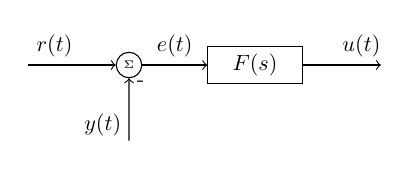
\begin{tikzpicture}[node distance=22mm, block/.style={rectangle, draw, minimum width=15mm}, sumnode/.style={circle, draw, inner sep=2pt},scale=0.8, every node/.style={scale=0.8}]

    \node[coordinate] (input) {};
    \node[sumnode, right of=input, node distance=16mm] (sum) {\tiny $\Sigma$};
    \node[block, right of=sum, node distance=20mm] (pid)  {$F(s)$};
    \node[coordinate, below of=sum, node distance=12mm] (feedback) {};
    \node[coordinate, right of=pid, node distance=20mm] (output) {};

    \draw[->] (input) -- node[above, pos=0.3] {$r(t)$} (sum);
    \draw[->] (sum) -- node[above] {$e(t)$} (pid);
    \draw[->] (pid) -- node[above, near end] {$u(t)$} (output);
    \draw[->] (feedback) -- node[left, near start] {$y(t)$} node[right, pos=0.95] {-} (sum);
  \end{tikzpicture}
\end{center}

\alert{Parallel form (ISA)}
\[   F(s) &= k_c\left( 1 + \frac{1}{\tau_i s} + \tau_d s\right) \]

\alert{Series form}
\[F(s) = K_c \left( \frac{ \tau_I s + 1}{\tau_I s} \right) (\tau_D s + 1) 
= \underbrace{\frac{K_c(\tau_I + \tau_D)}{\tau_I}}_{k_c} \left(1 + \frac{1}{\underbrace{(\tau_I + \tau_D)}_{\tau_i} s} + \underbrace{\frac{\tau_I\tau_D}{\tau_I + \tau_D}}_{\tau_d}s \right) \]
\end{frame}


\begin{frame}[label={sec:org288acd6}]{The PID - Parallel form}
\definecolor{ppc}{rgb}{0.1,0.1,0.6}
\definecolor{iic}{rgb}{0.6,0.1,0.1}
\definecolor{ddc}{rgb}{0.1,0.6,0.1}

\begin{center}
  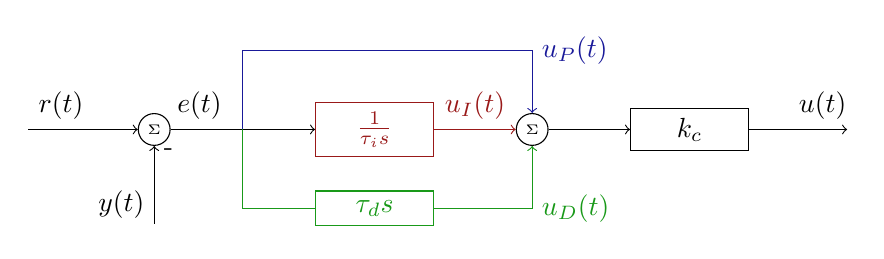
\begin{tikzpicture}[node distance=22mm, block/.style={rectangle, draw, minimum width=15mm}, sumnode/.style={circle, draw, inner sep=2pt}]

    \node[coordinate] (input) {};
    \node[sumnode, right of=input, node distance=16mm] (sum) {\tiny $\Sigma$};
    \node[color=iic,block, right of=sum, node distance=28mm] (ii)  {$\frac{1}{\tau_is}$};
    \node[color=ppc, coordinate, above of=ii, node distance=10mm] (pp)  {};
    \node[color=ddc,block, below of=ii, node distance=10mm] (dd)  {$\tau_ds$};
    \node[sumnode, right of=ii, node distance=20mm] (sum2) {\tiny $\Sigma$};
    \node[block, right of=sum2, node distance=20mm] (gain)  {$k_c$};
    \node[coordinate, below of=sum, node distance=12mm] (feedback) {};
    \node[coordinate, right of=gain, node distance=20mm] (output) {};

    \draw[->] (input) -- node[above, pos=0.3] {$r(t)$} (sum);
    \draw[->] (sum) -- node[above, pos=0.2] {$e(t)$} node[coordinate] (mm) {}  (ii);
    \draw[->] (gain) -- node[above, near end] {$u(t)$} (output);
    \draw[->] (feedback) -- node[left, near start] {$y(t)$} node[right, pos=0.95] {-} (sum);
    \draw[->, color=ppc] (mm) |- (pp) -| node[right,] {$u_P(t)$} (sum2);
    \draw[->, color=ddc] (mm) |- (dd) -| node[right,] {$u_D(t)$} (sum2);
    \draw[->, color=iic] (ii)  -- node[above,] {$u_I(t)$} (sum2);
    \draw[->] (sum2) -- node[above, near end] {} (gain);

  \end{tikzpicture}
\end{center}

\begin{align*}
u(t) &= k_c\Big( \textcolor{ppc}{e(t)} + \textcolor{iic}{\frac{1}{\tau_i} \int_0^{t} e(\xi) d\xi} + \textcolor{ddc}{\tau_d \frac{d}{dt} e(t)} \Big)
\end{align*}
\end{frame}

\begin{frame}[label={sec:org9114acc}]{The PID - Parallel form, modified D-part}
\definecolor{ppc}{rgb}{0.1,0.1,0.6}
\definecolor{iic}{rgb}{0.6,0.1,0.1}
\definecolor{ddc}{rgb}{0.1,0.6,0.1}

\begin{center}
  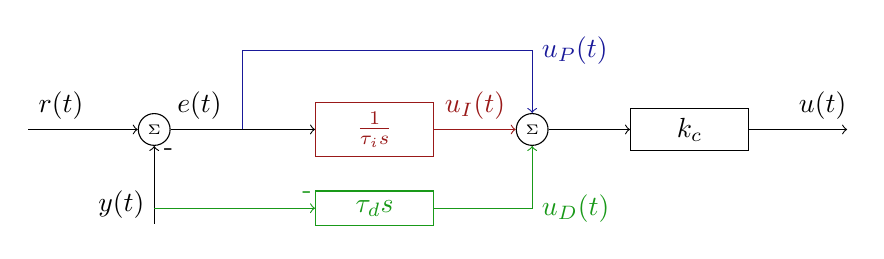
\begin{tikzpicture}[node distance=22mm, block/.style={rectangle, draw, minimum width=15mm}, sumnode/.style={circle, draw, inner sep=2pt}]

    \node[coordinate] (input) {};
    \node[sumnode, right of=input, node distance=16mm] (sum) {\tiny $\Sigma$};
    \node[color=iic,block, right of=sum, node distance=28mm] (ii)  {$\frac{1}{\tau_is}$};
    \node[color=ppc, coordinate, above of=ii, node distance=10mm] (pp)  {};
    \node[color=ddc,block, below of=ii, node distance=10mm] (dd)  {$\tau_ds$};
    \node[sumnode, right of=ii, node distance=20mm] (sum2) {\tiny $\Sigma$};
    \node[block, right of=sum2, node distance=20mm] (gain)  {$k_c$};
    \node[coordinate, below of=sum, node distance=12mm] (feedback) {};
    \node[coordinate, right of=gain, node distance=20mm] (output) {};

    \draw[->] (input) -- node[above, pos=0.3] {$r(t)$} (sum);
    \draw[->] (sum) -- node[above, pos=0.2] {$e(t)$} node[coordinate] (mm) {}  (ii);
    \draw[->] (gain) -- node[above, near end] {$u(t)$} (output);
    \draw[->] (feedback) -- node[left, near start] {$y(t)$} node[right, pos=0.95] {-} (sum);
    \draw[->, color=ppc] (mm) |- (pp) -| node[right,] {$u_P(t)$} (sum2);
    \draw[->, color=ddc] (feedback |- dd) -- node[above, pos=0.95] {-} (dd);
    \draw[->, color=ddc] (dd) -| node[right,] {$u_D(t)$} (sum2)  ;
    \draw[->, color=iic] (ii)  -- node[above,] {$u_I(t)$} (sum2);
    \draw[->] (sum2) -- node[above, near end] {} (gain);

  \end{tikzpicture}
\end{center}

\[    u(t) = k_c\Big( \textcolor{ppc}{e(t)} + \textcolor{iic}{\overbrace{\frac{1}{\tau_i} \int_0^{t} e(\xi) d\xi}^{u_I(t)}} + \textcolor{ddc}{ \underbrace{\tau_d \frac{d}{dt} \big(-y(t)\big)}_{u_D(t)}} \Big) \]
\end{frame}

\begin{frame}[label={sec:orga8d20ff}]{The PID - Parallel form}
\begin{center}
  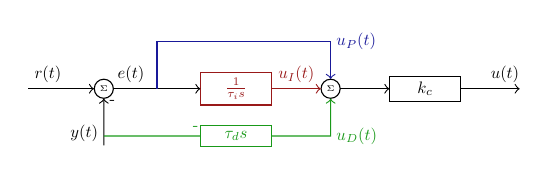
\begin{tikzpicture}[node distance=22mm, block/.style={rectangle, draw, minimum width=15mm}, sumnode/.style={circle, draw, inner sep=2pt}, scale=0.6, every node/.style={scale=0.6}]

    \node[coordinate] (input) {};
    \node[sumnode, right of=input, node distance=16mm] (sum) {\tiny $\Sigma$};
    \node[color=iic,block, right of=sum, node distance=28mm] (ii)  {$\frac{1}{\tau_is}$};
    \node[color=ppc, coordinate, above of=ii, node distance=10mm] (pp)  {};
    \node[color=ddc,block, below of=ii, node distance=10mm] (dd)  {$\tau_ds$};
    \node[sumnode, right of=ii, node distance=20mm] (sum2) {\tiny $\Sigma$};
    \node[block, right of=sum2, node distance=20mm] (gain)  {$k_c$};
    \node[coordinate, below of=sum, node distance=12mm] (feedback) {};
    \node[coordinate, right of=gain, node distance=20mm] (output) {};

    \draw[->] (input) -- node[above, pos=0.3] {$r(t)$} (sum);
    \draw[->] (sum) -- node[above, pos=0.2] {$e(t)$} node[coordinate] (mm) {}  (ii);
    \draw[->] (gain) -- node[above, near end] {$u(t)$} (output);
    \draw[->] (feedback) -- node[left, near start] {$y(t)$} node[right, pos=0.95] {-} (sum);
    \draw[->, color=ppc] (mm) |- (pp) -| node[right,] {$u_P(t)$} (sum2);
    \draw[->, color=ddc] (feedback |- dd) -- node[above, pos=0.95] {-} (dd) -| node[right,] {$u_D(t)$}   (sum2);
    \draw[->, color=iic] (ii)  -- node[above,] {$u_I(t)$} (sum2);
    \draw[->] (sum2) -- node[above, near end] {} (gain);

  \end{tikzpicture}
  \small
  \(  u(t) = k_c\Big( \textcolor{ppc}{e(t)} + \textcolor{iic}{\overbrace{\frac{1}{\tau_i} \int_0^{t} e(\xi) d\xi}^{u_I(t)}} + \textcolor{ddc}{ \underbrace{\tau_d \frac{d}{dt} \big(-y(t)\big)}_{u_D(t)}} \Big)\)
\end{center}

   \begin{center}
   \def\TT{1}
   \begin{tikzpicture}
   \begin{axis}[
    clip=false,
    width=14cm,
    height=4.2cm,
    ylabel={},
    xlabel={$t$},
    ymax = 2,
    ymin = -0.5,
    ]
      \addplot[black, no marks, domain=-0.1:8, samples=200] {(x>0)*(1 - (1+x/\TT)*exp(-x/\TT)} node[coordinate, pin=-20:{$y(t)$}, pos=0.4] {};
      \addplot[magenta!70!black, no marks, domain=-0.1:8, samples=200] coordinates {(-0.1, 0) (0,0) (0,1) (8,1)} node[coordinate, pin=90:{$r(t)$}, pos=0.4] {};
    \end{axis}

 \end{tikzpicture}
\end{center}
\alert{Activity} Sketch the error signal \(e(t)\), the derivative signal \(u_D(t)\) and the integral signal \(u_I(t)\) (use \(\tau_i=\tau_d=1\))
\end{frame}

\begin{frame}[label={sec:orgaea28f1}]{The PID - Parallel form, solution}
\end{frame}
\begin{frame}[label={sec:org192fa56}]{The PID - Parallel form, solution}
\(u(t) = k_c\Big( \textcolor{ppc}{e(t)} + \textcolor{iic}{\overbrace{\frac{1}{\tau_i} \int_0^{t} e(\xi) d\xi}^{u_I(t)}} + \textcolor{ddc}{ \underbrace{\tau_d \frac{d}{dt} \big(-y(t)\big)}_{u_D(t)}} \Big)\)
   \begin{center}
   \def\TT{1}
   \begin{tikzpicture}
   \begin{axis}[
    clip=false,
    width=14cm,
    height=5cm,
    ylabel={},
    xlabel={$t$},
    ymax = 2,
    ]
      \addplot[black, no marks, domain=-0.1:8, samples=200] {(x>0)*(1 - (1+x/\TT)*exp(-x/\TT)} node[coordinate, pin=-20:{$y(t)$}, pos=0.4] {};
      \addplot[magenta!70!black, no marks, domain=-0.1:8, samples=200] coordinates {(-0.1, 0) (0,0) (0,1) (8,1)} node[coordinate, pin=90:{$r(t)$}, pos=0.21] {};
      \addplot[color=ppc, no marks, domain=0:8, samples=200] {(x>=0)*( (1+x/\TT)*exp(-x/\TT)} node[coordinate, pin=20:{$e(t)$}, pos=0.7] {};
      \addplot[color=iic, no marks, domain=-0.1:8, samples=200] {(x>0)*(2*(1-exp(-x/\TT)) - \x/\TT*exp(-x/\TT))} node[coordinate, pin=-20:{$u_I(t)$}, pos=0.6] {};
      \addplot[color=ddc, no marks, domain=-0.1:8, samples=200] {(x>0)*(-\x/\TT*exp(-x/\TT))} node[coordinate, pin=-20:{$u_D(t)$}, pos=0.4] {};
    \end{axis}

 \end{tikzpicture}
\end{center}
\end{frame}

\begin{frame}[label={sec:org4816b36}]{The PID - practical form}
\definecolor{ppc}{rgb}{0.1,0.1,0.6}
\definecolor{iic}{rgb}{0.6,0.1,0.1}
\definecolor{ddc}{rgb}{0.1,0.5,0.1}

\begin{center}
  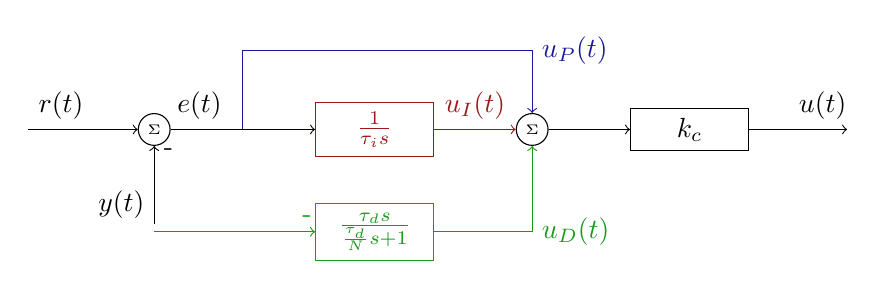
\begin{tikzpicture}[node distance=22mm, block/.style={rectangle, draw, minimum width=15mm}, sumnode/.style={circle, draw, inner sep=2pt}]

    \node[coordinate] (input) {};
    \node[sumnode, right of=input, node distance=16mm] (sum) {\tiny $\Sigma$};
    \node[color=iic,block, right of=sum, node distance=28mm] (ii)  {$\frac{1}{\tau_is}$};
    \node[color=ppc, coordinate, above of=ii, node distance=10mm] (pp)  {};
    \node[color=ddc,block, below of=ii, node distance=13mm] (dd)  {$\frac{\tau_ds}{\frac{\tau_d}{N}s + 1}$};
    \node[sumnode, right of=ii, node distance=20mm] (sum2) {\tiny $\Sigma$};
    \node[block, right of=sum2, node distance=20mm] (gain)  {$k_c$};
    \node[coordinate, below of=sum, node distance=12mm] (feedback) {};
    \node[coordinate, right of=gain, node distance=20mm] (output) {};

    \draw[->] (input) -- node[above, pos=0.3] {$r(t)$} (sum);
    \draw[->] (sum) -- node[above, pos=0.2] {$e(t)$} node[coordinate] (mm) {}  (ii);
    \draw[->] (gain) -- node[above, near end] {$u(t)$} (output);
    \draw[->] (feedback) -- node[left, near start] {$y(t)$} node[right, pos=0.95] {-} (sum);
    \draw[->, color=ppc] (mm) |- (pp) -| node[right,] {$u_P(t)$} (sum2);
    \draw[->, color=ddc] (feedback |- dd) -- node[above, pos=0.95] {-} (dd);
    \draw[->, color=ddc] (dd) -| node[right,] {$u_D(t)$} (sum2)  ;
    \draw[->, color=iic] (ii)  -- node[above,] {$u_I(t)$} (sum2);
    \draw[->] (sum2) -- node[above, near end] {} (gain);

  \end{tikzpicture}
\end{center}

The parameter \(N\) is chosen to limit the influence of noisy measurements. Typically,
\[  3 < N < 20 \]
\end{frame}

\section{PID tuning - (Smith and Corripio) Ziegler Nichols}
\label{sec:orgef9bf0d}
\begin{frame}[label={sec:orgc65ab9f}]{PID tuning}
\end{frame}
\begin{frame}[label={sec:org6cab308}]{Method by Smith \& Corripio using table by Ziegler-Nichols}
\small

Given process model (fitted to response of the system) \[ G(s) = K \frac{\mathrm{e}^{-s\theta}}{\tau s + 1} \] and PID controller
   \[ F(s) = k_c\left( 1 + \frac{1}{\tau_i s} + \tau_d s\right) \]
   Choose the PID parameters according to the following table (Ziegler-Nichols, 1943)
   \begin{center}
   \setlength{\tabcolsep}{20pt}
   \renewcommand{\arraystretch}{1.5}
   \begin{tabular}{llll}
   Controller & \(k_c\) & \(\tau_i\) & \(\tau_d\)\\
  \hline\hline
  P & \(\frac{\tau}{\theta K}\) &  & \\
  PI & \(\frac{0.9\tau}{\theta K}\) & \(\frac{\theta}{0.3}\) & \\
  PID & \(\frac{1.2\tau}{\theta K}\) & \(2\theta\) & \(\frac{\theta}{2}\)\\
  \hline
\end{tabular}
\end{center}

Gives good control for \[0.1 < \frac{\theta}{\tau} < 0.6.\]
\end{frame}

\section{Fitting first-order model with delay}
\label{sec:org5c3dc80}

\begin{frame}[label={sec:orgadb0320}]{Fitting first-order model with delay}
Assuming a plant model of first-order with time constant \(\tau\) and delay \(\theta\)
\[  \quad \textcolor{green!50!black}{Y(s)} = \frac{K\mathrm{e}^{-s\theta}}{s\tau + 1}\textcolor{blue!80!black}{U(s)} \quad \overset{U(s) = \frac{u_f}{s}}{\Longrightarrow} \quad \textcolor{green!50!black}{y(t)} = u_f K\big( 1 - \mathrm{e}^{-\frac{t-\theta}{\tau}}\big)u_H(t-\theta)\]
\def\Tcnst{3}
\def\tdelay{0.6}
\def\ggain{2}
\def\uampl{0.8}
\pgfmathsetmacro{\yfinal}{\uampl*\ggain}
\pgfmathsetmacro{\yone}{0.283*\yfinal}
\pgfmathsetmacro{\ytwo}{0.632*\yfinal}
\pgfmathsetmacro{\tone}{\tdelay + \Tcnst/3}
\pgfmathsetmacro{\two}{\tdelay + \Tcnst}

\begin{center}
  \begin{tikzpicture}
    \begin{axis}[
    width=14cm,
    height=4.5cm,
    grid = both,
    xtick = {0, \tdelay, \tone, \two},
    xticklabels = {0, $\theta$, $\theta+\frac{\tau}{3}$, $\theta + \tau$},
    ytick = {0, \yone, \ytwo, \uampl, \yfinal},
    yticklabels = {0, $ $, $ $, $u_f$, $y_f$},
    xmin = -0.2,
    %minor y tick num=9,
    %minor x tick num=9,
    %every major grid/.style={red, opacity=0.5},
    xlabel = {$t$},
    ]
      \addplot [thick, green!50!black, no marks, domain=0:10, samples=100] {\uampl*\ggain*(x>\tdelay)*(1 - exp(-(x-\tdelay)/\Tcnst)} node [coordinate, pos=0.9, pin=-90:{$y(t)$}] {};
      \addplot [const plot, thick, blue!80!black, no marks, domain=-1:10, samples=100] coordinates {(-1,0) (0,0) (0,\uampl) (10,\uampl)} node [coordinate, pos=0.9, pin=-90:{$u(t)$}] {};
    \end{axis}
  \end{tikzpicture}
\end{center}

\alert{Individual activity} Evaluate the response \(y(t)\) at the two time instants \(t=\theta + \frac{\tau}{3}\) and \(t=\theta + \tau\)!
\end{frame}


\begin{frame}[label={sec:org0049621}]{Fitting first-order model with delay}
Assuming a plant model of first-order with time constant \(\tau\) and delay \(\theta\)
\[  \quad \textcolor{green!50!black}{Y(s)} = \frac{K\mathrm{e}^{-s\theta}}{s\tau + 1}\textcolor{blue!80!black}{U(s)} \quad \overset{U(s) = \frac{u_f}{s}}{\Longrightarrow} \quad \textcolor{green!50!black}{y(t)} = u_f K\big( 1 - \mathrm{e}^{-\frac{t-\theta}{\tau}}\big)u_H(t-\theta)\]
\def\Tcnst{3}
\def\tdelay{0.6}
\def\ggain{2}
\def\uampl{0.8}
\pgfmathsetmacro{\yfinal}{\uampl*\ggain}
\pgfmathsetmacro{\yone}{0.283*\yfinal}
\pgfmathsetmacro{\ytwo}{0.632*\yfinal}
\pgfmathsetmacro{\tone}{\tdelay + \Tcnst/3}
\pgfmathsetmacro{\two}{\tdelay + \Tcnst}

\begin{center}
  \begin{tikzpicture}
    \begin{axis}[
    width=14cm,
    height=4.5cm,
    grid = both,
    xtick = {0, \tdelay, \tone, \two},
    xticklabels = {0, $\theta$, $\theta+\frac{\tau}{3}$, $\theta + \tau$},
    ytick = {0, \yone, \ytwo, \uampl, \yfinal},
    yticklabels = {0, $0.283y_{f}$, $0.632y_f$, $u_f$, $y_f$},
    xmin = -0.2,
    %minor y tick num=9,
    %minor x tick num=9,
    %every major grid/.style={red, opacity=0.5},
    xlabel = {$t$},
    ]
      \addplot [thick, green!50!black, no marks, domain=0:10, samples=100] {\uampl*\ggain*(x>\tdelay)*(1 - exp(-(x-\tdelay)/\Tcnst)} node [coordinate, pos=0.9, pin=-90:{$y(t)$}] {};
      \addplot [const plot, thick, blue!80!black, no marks, domain=-1:10, samples=100] coordinates {(-1,0) (0,0) (0,\uampl) (10,\uampl)} node [coordinate, pos=0.9, pin=-90:{$u(t)$}] {};
    \end{axis}
  \end{tikzpicture}
\end{center}

\[ y_f = \lim_{t\to\infty} y(t) = u_f K \quad \Rightarrow \quad K = \frac{y_f}{u_f}. \]
\end{frame}

\begin{frame}[label={sec:orgce08b4c}]{First-order model with delay - example}
\[  \quad Y(s) = \frac{K\mathrm{e}^{-s\theta}}{s\tau + 1}U(s) \quad \overset{U(s) = \frac{u_f}{s}}{\Longrightarrow} \quad y(t) = u_f K\big( 1 - \mathrm{e}^{-\frac{t-\theta}{\tau}}\big)u_s(t-\theta)\]
\def\Tcnst{2.1}
\def\tdelay{1}
\def\ggain{2}
\def\uampl{0.8}
\pgfmathsetmacro{\yfinal}{\uampl*\ggain}
\pgfmathsetmacro{\yone}{0.283*\yfinal}
\pgfmathsetmacro{\ytwo}{0.632*\yfinal}
\pgfmathsetmacro{\tone}{\tdelay + \Tcnst/3}
\pgfmathsetmacro{\two}{\tdelay + \Tcnst}

\begin{center}
  \begin{tikzpicture}
    \begin{axis}[
    width=12cm,
    height=4cm,
    grid = both,
    %xtick = {0, \tdelay, \tone, \two},
    %xticklabels = {0, $\theta$, $\theta+\frac{\tau}{3}$, $\theta + \tau$},
    %ytick = {0, \yone, \ytwo, \uampl, \yfinal},
    %yticklabels = {0, $0.283y_{f}$, $0.632y_f$, $u_f$, $y_f$},
    xmin = -0.2,
    minor y tick num=9,
    minor x tick num=9,
    every major grid/.style={red, opacity=0.5},
    %xlabel = {$t$},
    clip = false,
    ]
      \addplot [thick, green!50!black, smooth, no marks, domain=0:10, samples=16] {\uampl*\ggain*(x>\tdelay)*(1 - exp(-(x-\tdelay)/\Tcnst)} node [coordinate, pos=0.9, pin=-90:{$y(t)$}] {};
      \addplot [const plot, thick, blue!80!black, no marks, domain=-1:10, samples=100] coordinates {(-1,0) (0,0) (0,\uampl) (10,\uampl)} node [coordinate, pos=0.9, pin=-90:{$u(t)$}] {};
      \draw[thick, green!70!black, dashed] (axis cs: 10, \yfinal) -- (axis cs: -1, \yfinal, -0.9) node[left, anchor=east] {$y_f = \yfinal$}; 
      \draw[blue!70!black, dashed] (axis cs: 0, \uampl) -- (axis cs: -1, \uampl, -0.9) node[left, anchor=east] {$u_f = \uampl$}; 
    \end{axis}
  \end{tikzpicture}
\end{center}
\end{frame}

\begin{frame}[label={sec:orga70f7de}]{First-order model with delay - example}
\[  \quad Y(s) = \frac{K\mathrm{e}^{-s\theta}}{s\tau + 1}U(s) \quad \overset{U(s) = \frac{u_f}{s}}{\Longrightarrow} \quad y(t) = u_f K\big( 1 - \mathrm{e}^{-\frac{t-\theta}{\tau}}\big)u_s(t-\theta)\]
\def\Tcnst{2.1}
\def\tdelay{1}
\def\ggain{2}
\def\uampl{0.8}
\pgfmathsetmacro{\yfinal}{\uampl*\ggain}
\pgfmathsetmacro{\yone}{0.283*\yfinal}
\pgfmathsetmacro{\ytwo}{0.632*\yfinal}
\pgfmathsetmacro{\tone}{\tdelay + \Tcnst/3}
\pgfmathsetmacro{\two}{\tdelay + \Tcnst}

\begin{center}
  \begin{tikzpicture}
    \begin{axis}[
    width=12cm,
    height=4cm,
    grid = both,
    %xtick = {0, \tdelay, \tone, \two},
    %xticklabels = {0, $\theta$, $\theta+\frac{T}{3}$, $\theta + T$},
    %ytick = {0, \yone, \ytwo, \uampl, \yfinal},
    %yticklabels = {0, $0.283y_{f}$, $0.632y_f$, $u_f$, $y_f$},
    xmin = -0.2,
    minor y tick num=9,
    minor x tick num=9,
    every major grid/.style={red, opacity=0.5},
    %xlabel = {$t$},
    clip = false,
    ]
      \addplot [thick, green!50!black, smooth, no marks, domain=0:10, samples=16] {\uampl*\ggain*(x>\tdelay)*(1 - exp(-(x-\tdelay)/\Tcnst)} node [coordinate, pos=0.9, pin=-90:{$y(t)$}] {};
      \addplot [const plot, thick, blue!80!black, no marks, domain=-1:10, samples=100] coordinates {(-1,0) (0,0) (0,\uampl) (10,\uampl)} node [coordinate, pos=0.9, pin=-90:{$u(t)$}] {};
      \draw[thick, orange, dashed] (axis cs: \two, \ytwo) -- (axis cs: \two, -0.9) node[below] {$t_2 = \two = \theta + \tau$}; 
      \draw[thick, orange, dashed] (axis cs: \two, \ytwo) -- (axis cs: -1, \ytwo, -0.9) node[left, anchor=east] {$0.632y_f = \ytwo$}; 
      \draw[thick, green!70!black, dashed] (axis cs: 10, \yfinal) -- (axis cs: -1, \yfinal, -0.9) node[left, anchor=east] {$y_f = \yfinal$}; 
      \draw[blue!70!black, dashed] (axis cs: 0, \uampl) -- (axis cs: -1, \uampl, -0.9) node[left, anchor=east] {$u_f = \uampl$}; 
    \end{axis}
  \end{tikzpicture}
\end{center}
\end{frame}

\begin{frame}[label={sec:orge8ca517}]{First-order model with delay - example}
\[  \quad Y(s) = \frac{K\mathrm{e}^{-s\theta}}{s\tau + 1}U(s) \quad \overset{U(s) = \frac{u_f}{s}}{\Longrightarrow} \quad y(t) = u_f K\big( 1 - \mathrm{e}^{-\frac{t-\theta}{\tau}}\big)u_s(t-\theta)\]
\def\Tcnst{2.1}
\def\tdelay{1}
\def\ggain{2}
\def\uampl{0.8}
\pgfmathsetmacro{\yfinal}{\uampl*\ggain}
\pgfmathsetmacro{\yone}{0.283*\yfinal}
\pgfmathsetmacro{\ytwo}{0.632*\yfinal}
\pgfmathsetmacro{\tone}{\tdelay + \Tcnst/3}
\pgfmathsetmacro{\two}{\tdelay + \Tcnst}

\begin{center}
  \begin{tikzpicture}
    \begin{axis}[
    width=12cm,
    height=4cm,
    grid = both,
    %xtick = {0, \tdelay, \tone, \two},
    %xticklabels = {0, $\theta$, $\theta+\frac{T}{3}$, $\theta + T$},
    %ytick = {0, \yone, \ytwo, \uampl, \yfinal},
    %yticklabels = {0, $0.283y_{f}$, $0.632y_f$, $u_f$, $y_f$},
    xmin = -0.2,
    minor y tick num=9,
    minor x tick num=9,
    every major grid/.style={red, opacity=0.5},
    %xlabel = {$t$},
    clip = false,
    ]
      \addplot [thick, green!50!black, smooth, no marks, domain=0:10, samples=16] {\uampl*\ggain*(x>\tdelay)*(1 - exp(-(x-\tdelay)/\Tcnst)} node [coordinate, pos=0.9, pin=-90:{$y(t)$}] {};
      \addplot [const plot, thick, blue!80!black, no marks, domain=-1:10, samples=100] coordinates {(-1,0) (0,0) (0,\uampl) (10,\uampl)} node [coordinate, pos=0.9, pin=-90:{$u(t)$}] {};
      \draw[thick, red, dashed] (axis cs: \tone, \yone) -- (axis cs: \tone, -0.45) node[below] {$t_1 = \tone = \theta + \frac{\tau}{3}$}; 
      \draw[thick, red, dashed] (axis cs: \tone, \yone) -- (axis cs: -1,\yone) node[left, anchor=east] {$0.283y_f = \yone$}; 
      \draw[thick, orange, dashed] (axis cs: \two, \ytwo) -- (axis cs: \two, -0.9) node[below] {$t_2 = \two = \theta + \tau$}; 
      \draw[thick, orange, dashed] (axis cs: \two, \ytwo) -- (axis cs: -1, \ytwo, -0.9) node[left, anchor=east] {$0.632y_f = \ytwo$}; 
      \draw[thick, green!70!black, dashed] (axis cs: 10, \yfinal) -- (axis cs: -1, \yfinal, -0.9) node[left, anchor=east] {$y_f = \yfinal$}; 
      \draw[blue!70!black, dashed] (axis cs: 0, \uampl) -- (axis cs: -1, \uampl, -0.9) node[left, anchor=east] {$u_f = \uampl$}; 
    \end{axis}
  \end{tikzpicture}
\end{center}
\end{frame}

\begin{frame}[label={sec:org50ebc80}]{First-order model with delay - example}
\[  \quad Y(s) = \frac{K\mathrm{e}^{-s\theta}}{s\tau + 1}U(s) \quad \overset{U(s) = \frac{u_f}{s}}{\Longrightarrow} \quad y(t) = u_f K\big( 1 - \mathrm{e}^{-\frac{t-\theta}{\tau}}\big)u_s(t-\theta)\]
\def\Tcnst{2.1}
\def\tdelay{1}
\def\ggain{2}
\def\uampl{0.8}
\pgfmathsetmacro{\yfinal}{\uampl*\ggain}
\pgfmathsetmacro{\yone}{0.283*\yfinal}
\pgfmathsetmacro{\ytwo}{0.632*\yfinal}
\pgfmathsetmacro{\tone}{\tdelay + \Tcnst/3}
\pgfmathsetmacro{\two}{\tdelay + \Tcnst}

\begin{center}
  \begin{tikzpicture}
    \begin{axis}[
    width=12cm,
    height=4cm,
    grid = both,
    %xtick = {0, \tdelay, \tone, \two},
    %xticklabels = {0, $\theta$, $\theta+\frac{T}{3}$, $\theta + T$},
    %ytick = {0, \yone, \ytwo, \uampl, \yfinal},
    %yticklabels = {0, $0.283y_{f}$, $0.632y_f$, $u_f$, $y_f$},
    xmin = -0.2,
    minor y tick num=9,
    minor x tick num=9,
    every major grid/.style={red, opacity=0.5},
    %xlabel = {$t$},
    clip = false,
    ]
      \addplot [thick, green!50!black, smooth, no marks, domain=0:10, samples=16] {\uampl*\ggain*(x>\tdelay)*(1 - exp(-(x-\tdelay)/\Tcnst)} node [coordinate, pos=0.9, pin=-90:{$y(t)$}] {};
      \addplot [const plot, thick, blue!80!black, no marks, domain=-1:10, samples=100] coordinates {(-1,0) (0,0) (0,\uampl) (10,\uampl)} node [coordinate, pos=0.9, pin=-90:{$u(t)$}] {};
      \draw[thick, red, dashed] (axis cs: \tone, \yone) -- (axis cs: \tone, -0.45) node[below] {$t_1 = \tone = \theta + \frac{\tau}{3}$}; 
      \draw[thick, red, dashed] (axis cs: \tone, \yone) -- (axis cs: -1,\yone) node[left, anchor=east] {$0.283y_f = \yone$}; 
      \draw[thick, orange, dashed] (axis cs: \two, \ytwo) -- (axis cs: \two, -0.9) node[below] {$t_2 = \two = \theta + \tau$}; 
      \draw[thick, orange, dashed] (axis cs: \two, \ytwo) -- (axis cs: -1, \ytwo, -0.9) node[left, anchor=east] {$0.632y_f = \ytwo$}; 
      \draw[thick, green!70!black, dashed] (axis cs: 10, \yfinal) -- (axis cs: -1, \yfinal, -0.9) node[left, anchor=east] {$y_f = \yfinal$}; 
      \draw[blue!70!black, dashed] (axis cs: 0, \uampl) -- (axis cs: -1, \uampl, -0.9) node[left, anchor=east] {$u_f = \uampl$}; 
    \end{axis}
  \end{tikzpicture}
\end{center}
\[ \begin{cases} \tone = \theta + \frac{\tau}{3}\\ \two = \theta + \tau \end{cases} \quad \Rightarrow \quad \begin{cases} \theta = \tdelay \\ \tau = \Tcnst \end{cases}, \qquad  K = \frac{y_f}{u_f} = \frac{\yfinal}{\uampl} = \ggain \]
\end{frame}



\section{Analytical PID design}
\label{sec:orgb34fb58}

\begin{frame}[label={sec:org7cae885}]{Analytical PID design}
\end{frame}
\begin{frame}[label={sec:orgdf78a2d}]{Analytical PID design}
   \begin{center}
   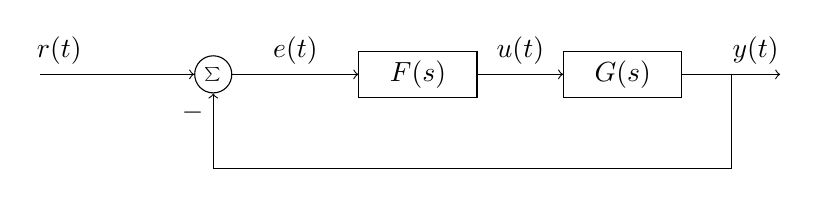
\begin{tikzpicture}[node distance=22mm, block/.style={rectangle, draw, minimum width=15mm}, sumnode/.style={circle, draw, inner sep=2pt}]
  { 
  \node[coordinate] (input) {};
  \node[sumnode, right of=input] (sum) {\tiny $\sum$};
  \node[block, right of=sum, node distance=2.6cm] (reg) {$F(s)$};
  \node[block, right of=reg, node distance=2.6cm] (plant) {$G(s)$};
  \node[coordinate, right of=plant, node distance=2cm] (output) {};
  \node[coordinate, below of=plant, node distance=12mm] (feedback) {};
 
  \draw[->] (plant) -- node[coordinate, inner sep=0pt] (meas) {} node[near end, above] {$y(t)$} (output);
  \draw[->] (meas) |- (feedback) -| node[very near end, left] {$-$} (sum);
  \draw[->] (input) -- node[very near start, above] {$r(t)$} (sum);
  \draw[->] (sum) -- node[above] {$e(t)$} (reg);
  \draw[->] (reg) -- node[above] {$u(t)$}(plant);
}
\end{tikzpicture}
\end{center}

\alert{Activity}  Solve for \(F(s)\) in the closed-loop transfer function \[G_c(s) = \frac{G(s)F(s)}{1 + G(s)F(s)}\] 
\end{frame}

\begin{frame}[label={sec:org3a440f1}]{Analytical PID design - Solution}
\end{frame}
\begin{frame}[label={sec:orgd79c818}]{Analytical PID design - Solution}
Solving for \(F(s)\) in the closed-loop transfer function \(G_c(s) = \frac{G(s)F(s)}{1 + G(s)F(s)}\) 

\[ \big(1 + G(s)F(s)\big) G_c(s) = G(s)F(s)\]
\[ G_c(s) = \big( 1 - G_c(s)\big) G(s)F(s)\]
\[F(s) = \frac{\frac{G_c(s)}{G(s)}}{1 - G_c(s)}\]
\end{frame}

\begin{frame}[label={sec:org5fee8ef}]{Analytic PID tuning - first-order with delay}
   \begin{center}
   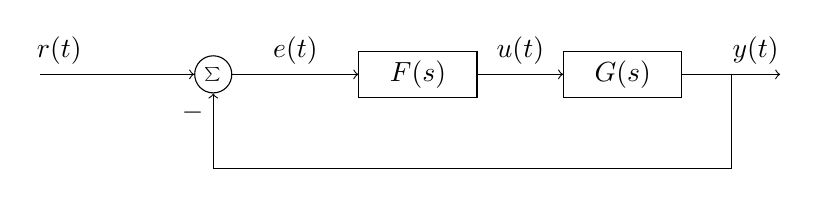
\begin{tikzpicture}[node distance=22mm, block/.style={rectangle, draw, minimum width=15mm}, sumnode/.style={circle, draw, inner sep=2pt}]
  { 
  \node[coordinate] (input) {};
  \node[sumnode, right of=input] (sum) {\tiny $\sum$};
  \node[block, right of=sum, node distance=2.6cm] (reg) {$F(s)$};
  \node[block, right of=reg, node distance=2.6cm] (plant) {$G(s)$};
  \node[coordinate, right of=plant, node distance=2cm] (output) {};
  \node[coordinate, below of=plant, node distance=12mm] (feedback) {};
 
  \draw[->] (plant) -- node[coordinate, inner sep=0pt] (meas) {} node[near end, above] {$y(t)$} (output);
  \draw[->] (meas) |- (feedback) -| node[very near end, left] {$-$} (sum);
  \draw[->] (input) -- node[very near start, above] {$r(t)$} (sum);
  \draw[->] (sum) -- node[above] {$e(t)$} (reg);
  \draw[->] (reg) -- node[above] {$u(t)$}(plant);
}
\end{tikzpicture}
\end{center}

Given model \(G(s) = K \frac{\mathrm{e}^{-s\theta}}{\tau s + 1}\) of the process and desired closed-loop transfer function \(G_c(s) = \frac{\mathrm{e}^{-s\theta}}{\tau_c s + 1}\)

\alert{Activity}  Show that the controller becomes
\[ F(s) = \frac{1}{K} \left( \frac{\tau s + 1}{\tau_c s + 1 - \mathrm{e}^{-s\theta}} \right) \approx \frac{1}{K} \left( \frac{\tau s + 1}{(\tau_c+\theta) s}\right)  = \underbrace{\frac{\tau}{K(\tau_c+\theta)}}_{k_c} \left( 1 + \frac{1}{\underbrace{\tau}_{\tau_i} s} \right).\]
Which is a PI-controller with \(k_c = \frac{\tau}{K(\tau_c+\theta)}\) and \(\tau_i = \tau\).
\end{frame}

\begin{frame}[label={sec:org0d28ec6}]{Example}
\small

   \begin{center}
   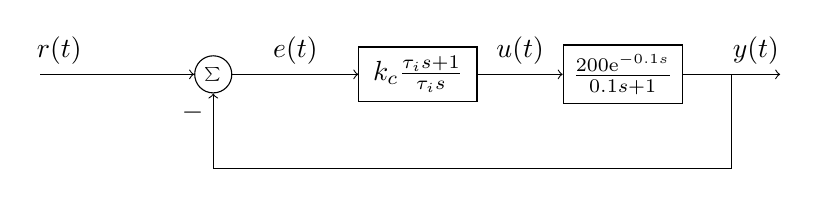
\begin{tikzpicture}[node distance=22mm, block/.style={rectangle, draw, minimum width=15mm}, sumnode/.style={circle, draw, inner sep=2pt}]
  { 
  \node[coordinate] (input) {};
  \node[sumnode, right of=input] (sum) {\tiny $\sum$};
  \node[block, right of=sum, node distance=2.6cm] (reg) {$k_c\frac{\tau_i s + 1}{\tau_i s}$};
  \node[block, right of=reg, node distance=2.6cm] (plant) {$\frac{200 \mathrm{e}^{-0.1s}}{0.1s + 1}$};
  \node[coordinate, right of=plant, node distance=2cm] (output) {};
  \node[coordinate, below of=plant, node distance=12mm] (feedback) {};
 
  \draw[->] (plant) -- node[coordinate, inner sep=0pt] (meas) {} node[near end, above] {$y(t)$} (output);
  \draw[->] (meas) |- (feedback) -| node[very near end, left] {$-$} (sum);
  \draw[->] (input) -- node[very near start, above] {$r(t)$} (sum);
  \draw[->] (sum) -- node[above] {$e(t)$} (reg);
  \draw[->] (reg) -- node[above] {$u(t)$}(plant);
}
\end{tikzpicture}
\end{center}

\(k_c = \frac{\tau}{K(\tau_c+\theta)}\) and \(\tau_i = \tau\).

\alert{Activity} Determine the controller for the choice \(\tau_c = \tau\)
\end{frame}
\end{document}